\chapter{Implementacja}
W tym rozdziale przedstawiono szczegóły implementacji systemu. 
Poszczególne zagadnienia oraz aplikacje wchodzące w jego skład
zostały opisane w oddzielnych sekcjach tego rozdziału.

\section{Komunikacja między warstwami}
Komunikacja między warstwami aplikacji odbywa się z wykorzystaniem protokołu 
HTTP (ang. \textit{Hypertext Transfer Protocol}).
Jest to jedna z technologii wykorzystywana w modelu TCP/IP 
nazywanego również protokołem Internetowym (ang. \textit{Internet Protocol}).
Jest protokołem bezstanowym \cite{http:rfc9110} służącym do przesyłania
informacji w postaci hipertekstowej i jest podstawowym rozwiązaniem
stosowanym w sieci WWW (ang. \textit{World Wide Web}), będąca systemem 
służącym do udostępniania informacji poprzez sieć Internet
z wykorzystaniem adresów URI (ang. \textit{Uniform Resource Identifier}) \cite{Jacobs:04:AWW}.

Dodatkowo wykorzystany został protokół kanałów komunikacyjnych WebSocket.
Pracują one w trybie pełnego dupleksu, co zezwala na obustronną komunikację
klienta z serwerem oraz serwera z klientem. Największą jego zaletą jest
możliwość wykorzystania protokołu HTTP w celu ustanowienia połączenia 
oraz wykorzystanie tych samych portów 80 oraz 443.
Aby ustanowić połączenie klient powinien wysłać odpowiedni
nagłówek nazywany HTTP Upgrade, na który serwer odpowiada z informacją o zmianie protokołu.
Następnie połączenie zmienia protokół z HTTP do binarnej transmisji bezpośrednio wykorzystującej TCP.
W tym momencie obie strony z jego wykorzystaniem mogą odczytywać oraz wysyłać wiadomości
pomiędzy sobą.

\section{Aplikacja serwerowa}
Aplikacja serwerowa została zaimplementowana jako centralny komponent systemu.
Zajmuje się zapisem odczytów w bazie danych, przetwarzaniem zapytań
pozostałych warstw, klienckiej oraz urządzeń pomiarowych,
poprzez wykorzystanie różnych metod HTTP.
Metoda POST zajmuje używana jest w nim do przekazywania danych
dla serwera w procesach takich jak tworzenie konta użytkownika,
wysyłanie nowego odczytu czy uwierzytelnianie.
Aplikacja następnie przetwarza te zapytanie oraz w odpowiedni 
sposób na nie reaguje, np. zapisując je na stałe do bazy danych 
lub wysyłając notyfikację użytkownikowi, po czym odpowiada
odpowiednim statusem klientowi.
Kolejną szeroko zastosowaną metodą jest GET. Służy ona do pobierania
zasobów z serwera. Klient wykorzystuje odpowiedni adres URI z
podstawowymi danymi lub bez, pod który wykonuje zapytanie, a
następnie serwer zwraca odpowiedź z zażądanymi informacjami.
Metodami służącymi do modyfikacji zasobów są PUT oraz DELETE.
Pierwsza z nich wykorzystywana jest do zmieniania istniejących
już zasobów lub tworzenia ich na nowo. DELETE natomiast służy
do usuwania zasobów.

Kolejnym zadaniem tej aplikacji jest również przechowywanie oraz synchronizacja konfiguracji
między pozostałymi urządzeniami w systemie. Użytkownik może ustawić podstawowe
parametry aplikacji takie jak graniczne wartości odczytów lub
częstotliwość pobierania odczytów z sensorów po czym te ustawienia
synchronizowane są z pozostałymi urządzeniami systemu.

Całość została wykonana z użyciem technologii ASP.NET Core.
Ułatwiło to znacznie implementację ze względu na bogate zasoby
tego środowiska ułatwiające pracę z protokołem HTTP oraz mnogość
bibliotek oraz wcześniej wykonanych projektów i przykładów z użyciem
tej technologii. 
Pierwszym z takich dodatkowych rozwiązań jest oficjalny sterownik
baz danych MongoDB dla środowiska .NET. Jego wykorzystanie 
umożliwiło na prostą interakcję między aplikacją oraz bazą
danych. Zamiast ręcznie dokonywać połączenia oraz przesyłać
komendy możliwa jest interakcja poprzez udostępniony interfejs.
Umożliwia on na wykorzystanie zaawansowanych technik takich jak
LINQ co znacznie ułatwiło tworzenie zapytań. Technologia ta
pomaga również w mapowaniu obiektów baz danych na klasy języka C\#.
W większości przypadków takie zależności tworzone są automatycznie,
jedynie w przypadku nadmiarowych lub braku wymaganych danych potrzebna
jest interakcja programisty. Przykładem z implementacji jest wymaganie
mapowania klas dziedziczących.
\begin{lstlisting}[language={[Sharp]C}]
BsonClassMap.RegisterClassMap<BaseUser>(cm =>
{
    cm.AutoMap();
    cm.AddKnownType(typeof(Device));
    cm.AddKnownType(typeof(User));
});
\end{lstlisting}
W tym odcinku kodu tworzona jest mapa automatyczna dla klasy BaseUser - podstawowej
użytkownika, a następnie wiązane są z nią dwa typy pochodne - Device, czyli urządzenie
oraz User, czyli użytkownik. Pozwala to na dostęp do obu typów użytkownika
z jednego kontekstu bazy danych.

Wykorzystanie ASP.NET ułatwiło również wykonanie systemu autoryzacji. 
Pakiet Microsoft.AspNetCore.Authentication zawiera często wykorzystywane metody
uwierzytelniania użytkowników. W implementacji aplikacji użyto metody tokenów JWT
(ang. \textit{JSON Web Token}). Jest to krótka, zakodowana w systemie Base64, 
reprezentacja uprawnień użytkownika używana w środowiskach z ograniczoną przestrzenią 
takich jak HTTP\cite{jwt:rfc7519}. Oprócz tego zawiera informacje o
czasie jego przedawnienia, audiencji oraz emitenta. Dzięki temu
może zostać wykorzystany w systemach pojedynczego logowania
SSO (ang. \textit{Single sign-on}) i wykorzystywany poprzez wiele aplikacji.
W implementacji został wykorzystany algorytm HmacSha256 do cyfrowego
podpisywania ważności tokenu. Sterowanie innymi parametrami takimi jak czas
przedawnienia, audiencja orz emitent odbywa się za pomocą edytowalnych
plików konfiguracyjnych.
\begin{lstlisting}[language={[Sharp]C}]
var token = new JwtSecurityToken(
  config["Issuer"],
  config["Audience"],
  claims,
  expires: DateTime.Now.Add(expiration),
  signingCredentials: new SigningCredentials(
    new SymmetricSecurityKey(Encoding.UTF8.GetBytes(config["SecretKey"])),
  SecurityAlgorithms.HmacSha256));
\end{lstlisting} 
Hasła użytkowników przechowywane są po wcześniejszym zakodowaniu algorytmem SHA256
z dodatkowymi informacjami nazywanymi solą. Są to losowe dane, które pozwalają na
dodatkowe zabezpieczenie kluczy przed wykryciem duplikatów lub ataków słownikowych
\cite{anderson2020security}.
Aby odpowiednio przejść proces uwieżytleniania użytkownik musi przesłać
swoją nazwę użytkownika oraz hasło zapytaniem z metodą POST pod odpowiedni adres
URI. Następnie jeżeli dane są prawidłowe w odpowiedzi otrzyma on wartość
token, która następnie może wykorzystać do dostępu do zablokowanych anonimowym
użytkownikom zasobów, takich jak tworzenie nowych odczytów. Wartość
ta musi zostać przesłana w nagłówku Authorization.
Użytkownicy dzielą się na różne role: administrator, użytkownik oraz urządzenie.
Administrator ma dostęp do wszystkich opcji aplikacji - konfiguracji, zarządzania odczytami
oraz użytkownikami, przeglądanie zasobów. Urządzenie może zarządzać jedynie swoimi
danymi, a zwykły użytkownik nie ma dostępu do edycji zasobów i może jedynie przeglądać
wartości.

Jako szkielet logiki aplikacji został wykorzystany wzorzec CQRS 
(ang. \textit{Command Query Responsibility Separation}).
W tym modelu akcje dzielą się na dwa typy komendy oraz zapytania \cite{fowler:cqrs}.
Komendy służą do interakcji z systemem, np. tworzenie użytkowników.
Mogą zawierać dodatkową logikę jak weryfikacja danych wejściowych 
czy sprawdzanie duplikatów.
Zapytania spełniają funkcję dostępu do danych. Pobierane oraz
filtrowane są w nich informacje z systemu i w razie potrzeby
odpowiednio transformowane.
Dzięki stosowaniu się do zasad tej metodyki aplikacja wolna
jest od efektów ubocznych i tworzenie zapytań nie zmienia
wartości systemu. Pozwala również na uproszczenie logiki
aplikacji ze względu na podział na proste moduły oraz bardzo
dobrą skalowalność z rozwiązaniami wielowątkowymi.
W implementacji tej metodyki wykorzystano bibliotekę MediatR.
Udostępnia ona bardzo łatwy w użyciu wzorzec mediatora.
Pozwala on na redukcję zależności między komponentami poprzez
zastosowanie centralnego obiektu zajmującego się komunikacją między nimi\cite{freeman2004head}.
W tym przypadku komponentami są komendy oraz zapytania i do ich realizacji
została wykorzystana dynamiczna implementacja centralnego
mediatora z biblioteki MediatR. Oddziela to dane od implementacji
zachowań i pozwala na ich niezależną modyfikacje.

Serwis notyfikacji został zaimplementowany z użyciem wzorca dekorator.
Jest to wzorzec projektowy pozwalający na dynamiczne dodawanie nowego
zachowania obiektowi bez modyfikacji innych obiektów tej samej klasy
\cite{freeman2004head}. Tym samym ułatwia on dostosowanie się do zasady
pojedynczej odpowiedzialności (ang. \textit{Single responsibility principle})
poprzez wydzielenie logiki na klasy zajmujące się tylko jednym zadaniem.
Jego wykorzystanie oznacza również zastosowanie zasady otwarte-zamknięte, w
której części systemu powinny być otwarte na rozszerzanie, ale zamknięte
na modyfikacje \cite{meyer1988object}. Jest to możliwe, gdyż dekorator pozwala
na dodanie nowych funkcjonalności obiektowi bez jego ponownego tworzenia.
Z jego wykorzystaniem użytkownik jest w stanie skonfigurować system notyfikacji,
aby ten wysyłał powiadomienia do różnych celów takich jak poczta elektroniczna
czy powiadomienia SMS.

Reguły sterujące logiką wysyłania powiadomień zbudowane zostały przy użyciu systemu
ekspresji środowiska .NET. Dzięki temu użytkownik może w rozbudowany sposób
tworzyć logikę określającą przy jakich warunkach powinna być wysłana dana wiadomość.
Dzięki temu, że są one kompilowane podczas wykonywania programu mogą przyjąć dowolną
formę, więc nie ograniczają użytkownika w ich tworzeniu oraz modyfikacji.
Serializacja oraz de-serializacja ekspresji została wykonana przy użyciu biblioteki
Serialize.Linq pozwalająca na ich zapis oraz odczyt do różnych formatów takich jak
JSON czy XML, które następnie przechowywane są w bazie danych.

Aby ułatwić implementację pozostałych aplikacji oraz w celu zapewnienia dokumentacji
wykorzystano bibliotekę Swashbuckle. Dostarcza ona składniki takie jak 
\begin{itemize}
  \item generator schematów OpenAPI, które mogą być następnie wykorzystane do generowania klientów
wykorzystujących dane API,
  \item generator dokumentacji bazujący na komentarzach znajdujących się w kodzie aplikacji,
  \item interfejs swagger-ui umożliwiający na przeglądanie zasobów z poziomu przeglądarki internetowej.
\end{itemize}
Interfejs swagger-ui przedstawiono na Rys. \ref{swagger:interface}.
\begin{figure}[h!]
  \centering
  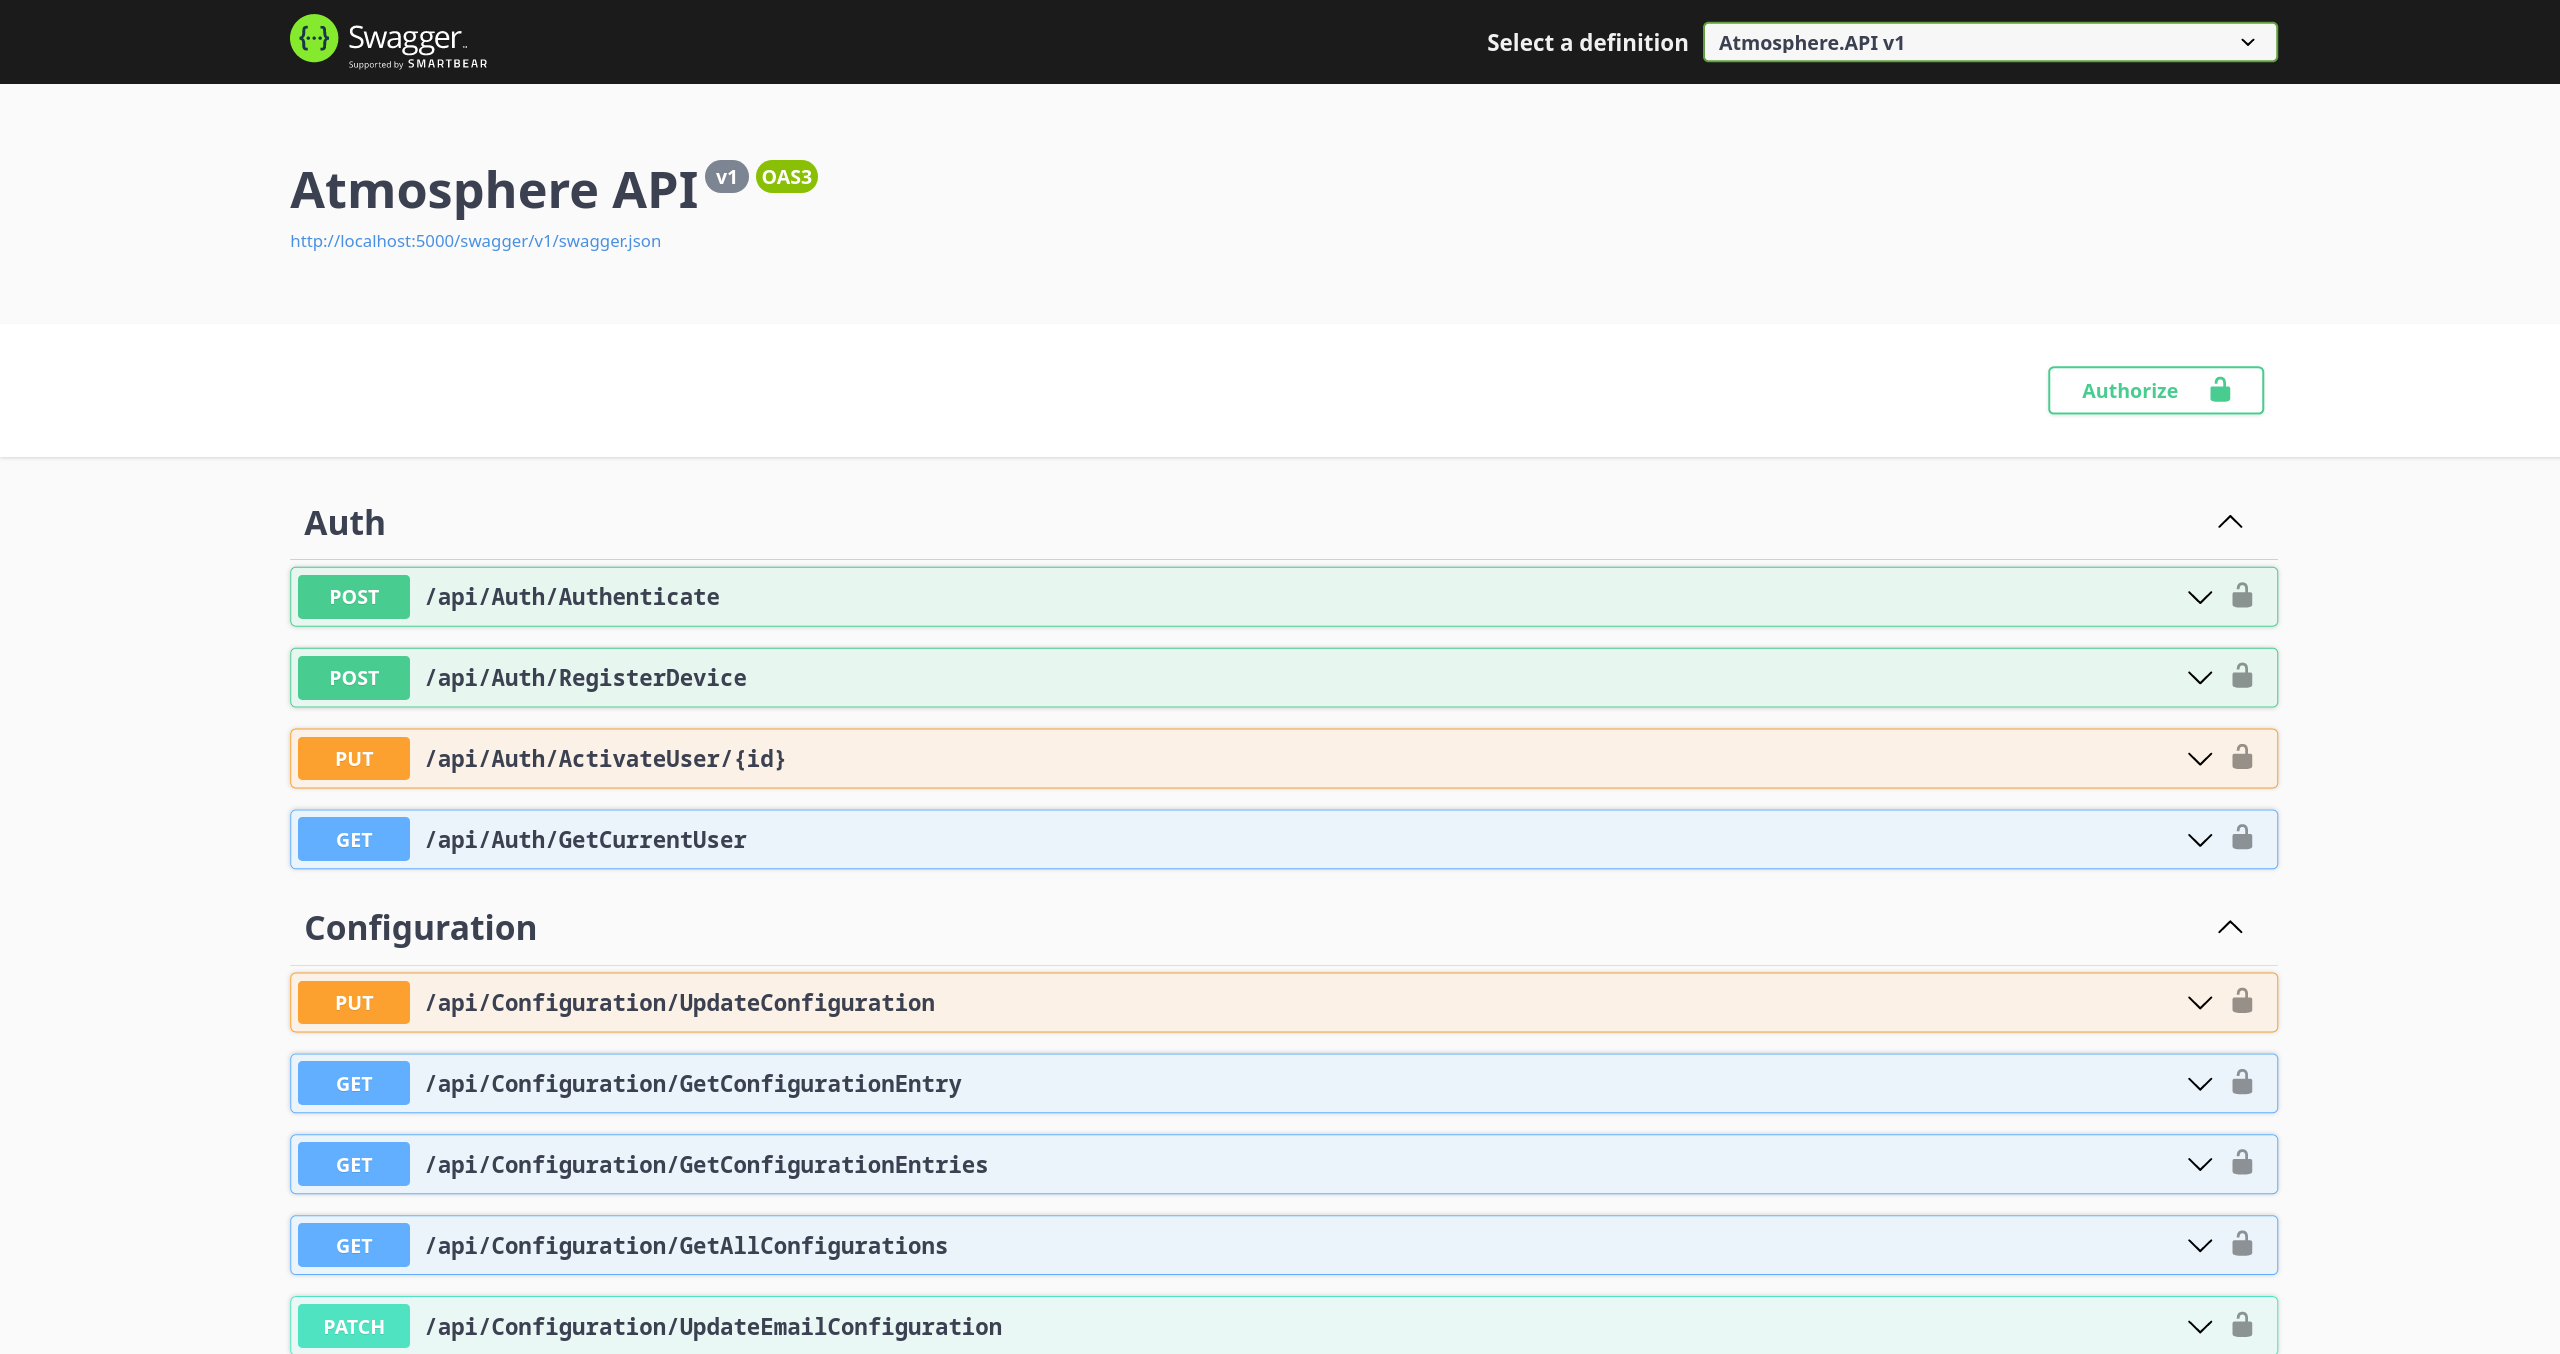
\includegraphics[width=\textwidth]{swagger}
  \caption{Intefejs swagger-ui}
  \label{swagger:interface}
\end{figure}
Kod wygenerowany na podstawie schematów wygenerowanych przez tą bibliotekę został następnie
wykorzystany zarówno w aplikacji klienckiej jak i urządzeniach pomiarowych.
Wykorzystano do tego oprogramowanie openapi-generator wspierające wiele języków
programowania oraz różnych bibliotek służących do komunikacji z użyciem protokołu HTTP.
Jest ono w stanie, na podstawie schematów OpenAPI, utworzyć klienta wraz z odpowiednimi
modelami jak również trzon aplikacji serwerowej oraz dokumentację. Pozwala również
na modyfikowanie wzorów generowanego kodu poprzez pliku mustache, za pomocą których
definiowana jest struktura wygenerowanych plików.

Pozostałe aplikacje w systemie mogą komunikować się z serwerem poprzez wykorzystanie
zapytań do odpowiednich kontrolerów. Zależnie od punktu końcowego muszą one
przesłać odpowiednie informacje w postaci ciała, ciągu lub argumentu pozycyjnego
zapytania. Aplikacja zawiera 3 główne kontrolery zajmujące się odpowiednim im zadaniom:
\begin{itemize}
  \item zapis oraz odczyt parametrów środowiska,
  \item autoryzacja oraz tworzenie kont,
  \item konfiguracja oraz pobieranie konfiguracji systemu,
  \item pobieranie szczegółowych danych o urządzeniach oraz ich statusie.
\end{itemize}
W celu ułatwienia obsługi każdy z kontrolerów znajduje się na ścieżce URI odpowiadającej
jego nazwie, np. kontroler odczytów znajduje się pod ścieżką /api/Reading.
Dodatkowo serwer udostępnia dwa połączenia WebSocket - notyfikacyjne oraz
dla urządzeń. Pierwsze z gniazd wykorzystywane jest do przesyłania
powiadomień do pozostałych aplikacji. Autoryzowani użytkownicy mogą
się z nim połączyć, aby uzyskać dostęp do wiadomości o niespodziewanych
wartościach odczytów parametrów środowiska. Gniazdo przeznaczone dla
urządzeń służy natomiast do synchronizacji konfiguracji oraz
udostępnienia statusu. Wszystkie połączenia powinny co 30 sekund
wysyłać wiadomość z zawartością "ping", aby zapewnić stałość połączenia.
W przeciwnym wypadku serwer uznaje połączenie za przerwane i zamyka je.
Wykorzystywane są one również do udostępniania notyfikacji oraz
synchronizacji konfiguracji z pozostałymi urządzeniami.

\section{Aplikacja kliencka}
Aplikacja kliencka powstała w celu ułatwienia dostępu do zasobów systemu.
Umożliwia ona na przedstawienie danych związanych z odczytami jak i konfigurację
aplikacji wykorzystując przyjazny użytkownikowi interfejs. W tym celu komunikuje
się ona z serwerem i na podstawie otrzymanych danych przedstawia je w formacie
czytelnym dla człowieka. 

Pierwszym krokiem, który wykonuje użytkownik po uruchomieniu aplikacji jest 
proces logowania. Aby zwiększyć bezpieczeństwo danych wszystkie funkcjonalności
dostępne są jedynie aktywnym kontom użytkowników.
Interfejs logowania przedstawiono na Rys. \ref{atmosphere:signin}.
\begin{figure}[h!]
  \centering
  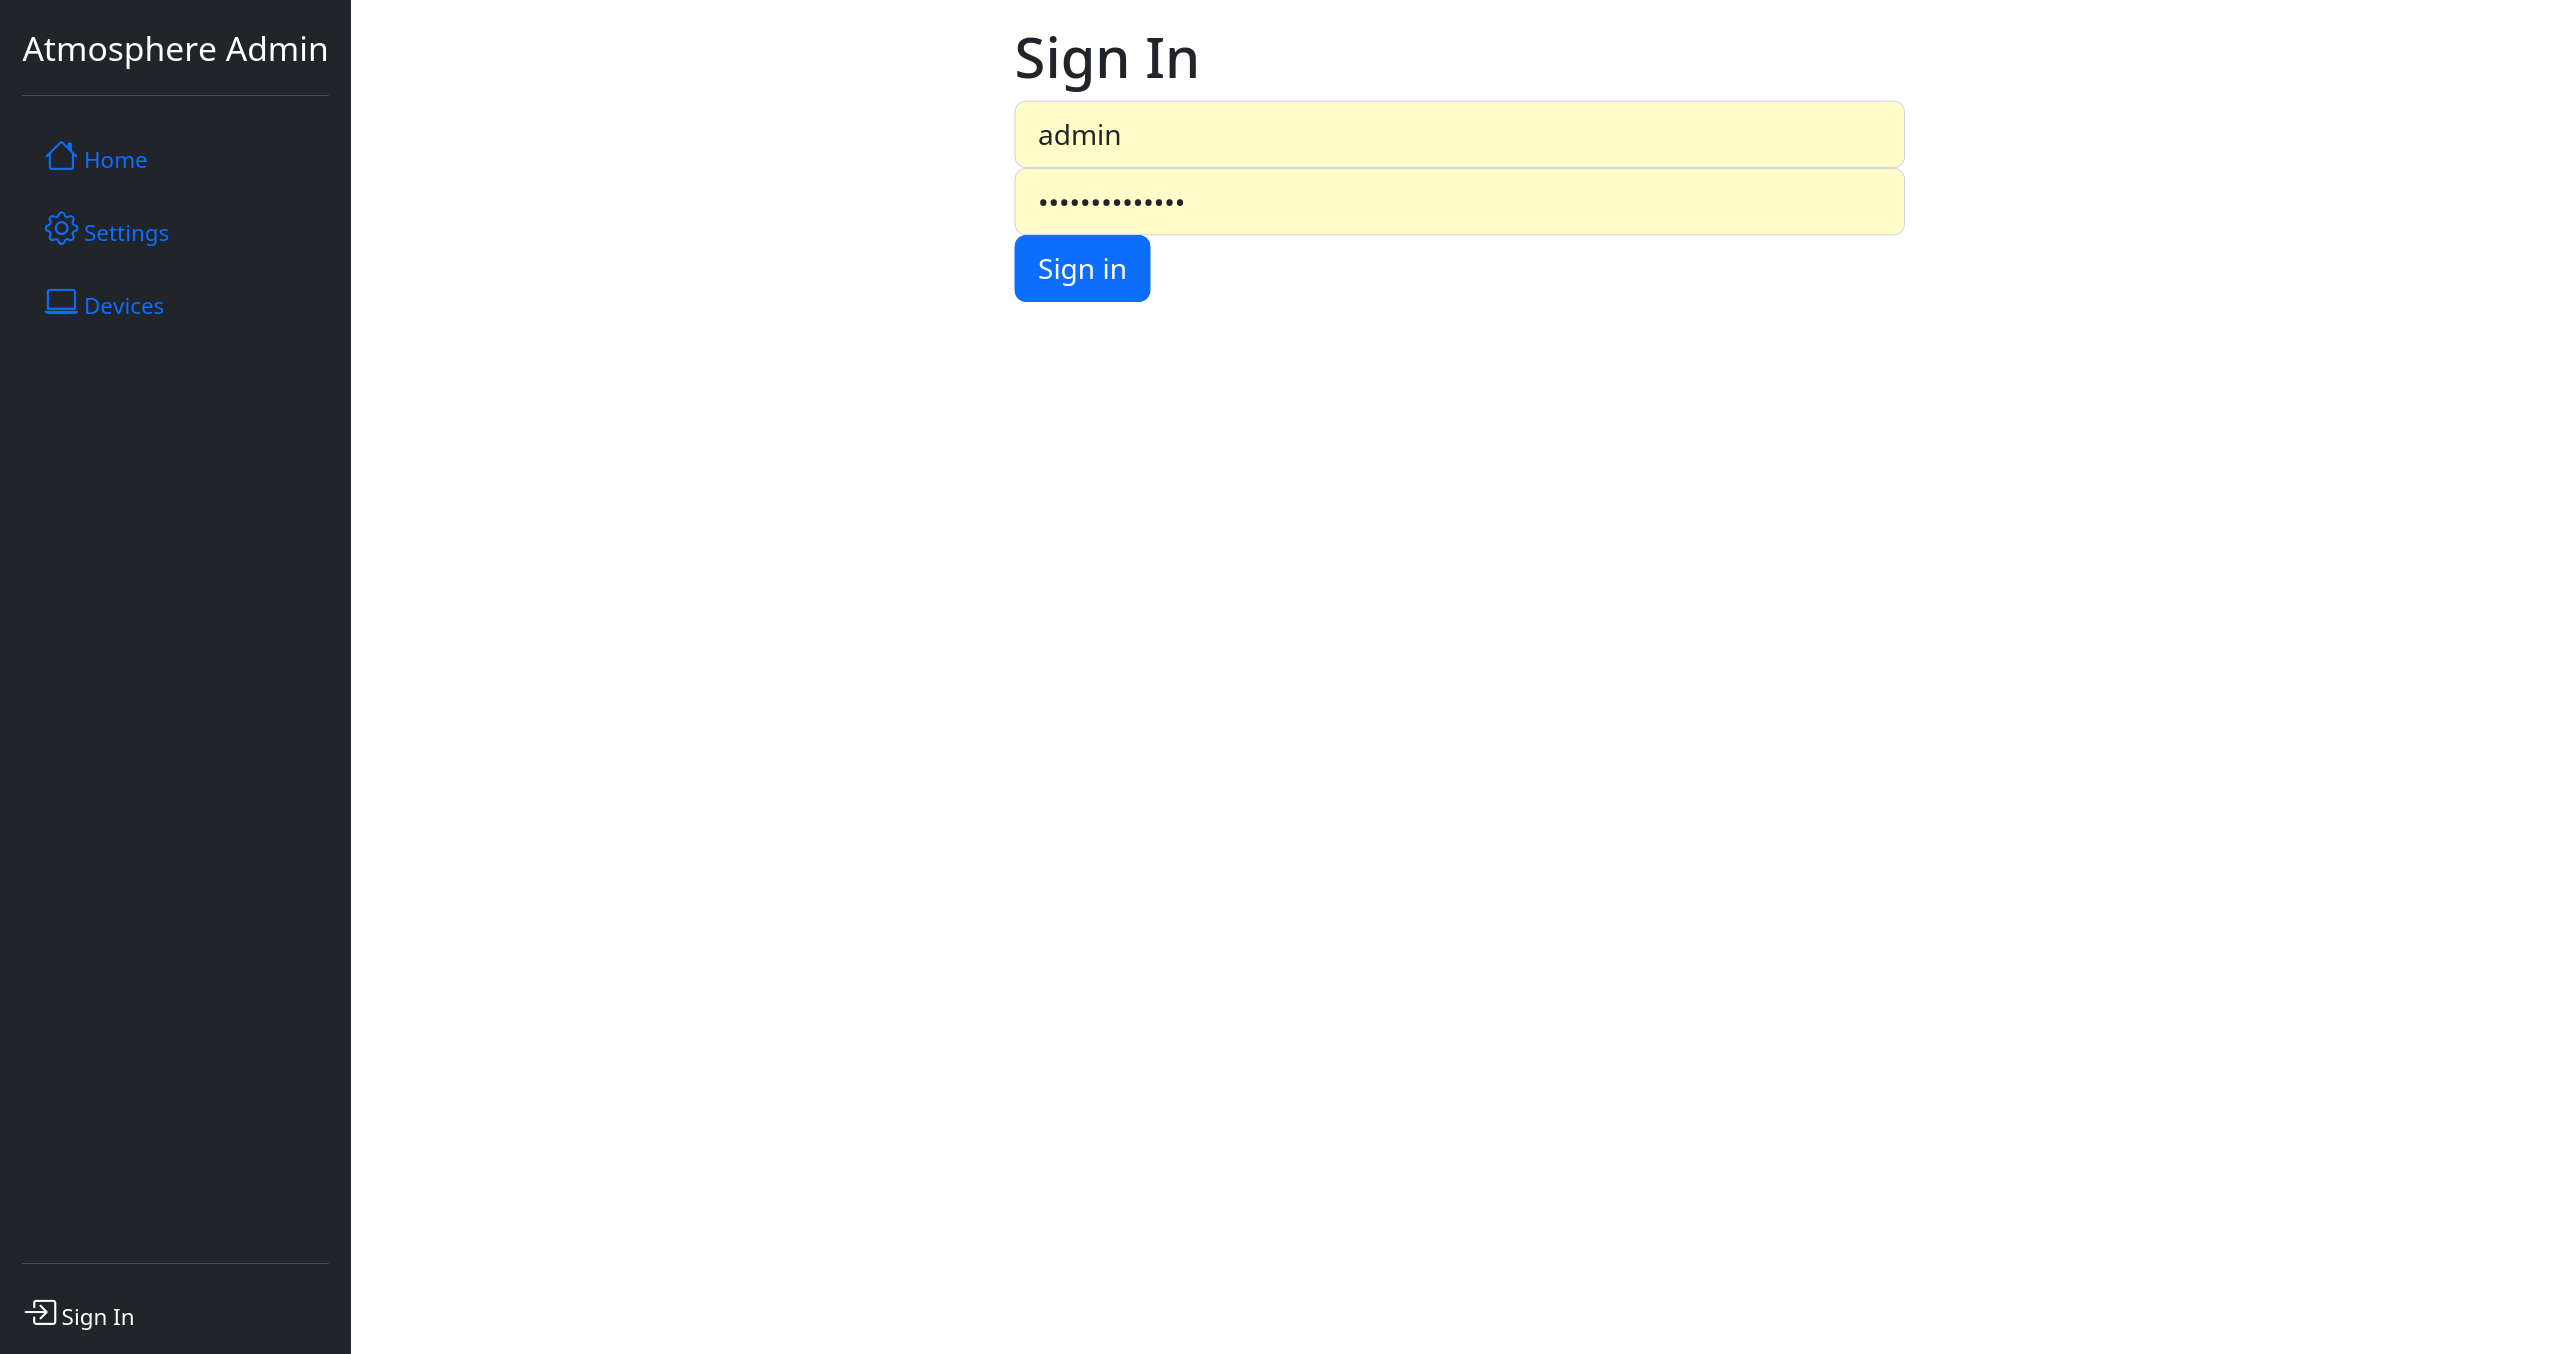
\includegraphics[width=\textwidth]{signin}
  \caption{Widok logowania}
  \label{atmosphere:signin}
\end{figure}
W przypadku podania błędnych danych serwer zwraca informację o błędzie, która następnie
wyświetlana jest w formie powiadomienia użytkownikowi. Przykładową zawartość przedstawiono
na Rys. \ref{atmosphere:failedsignin}.
\begin{figure}[h!]
  \centering
  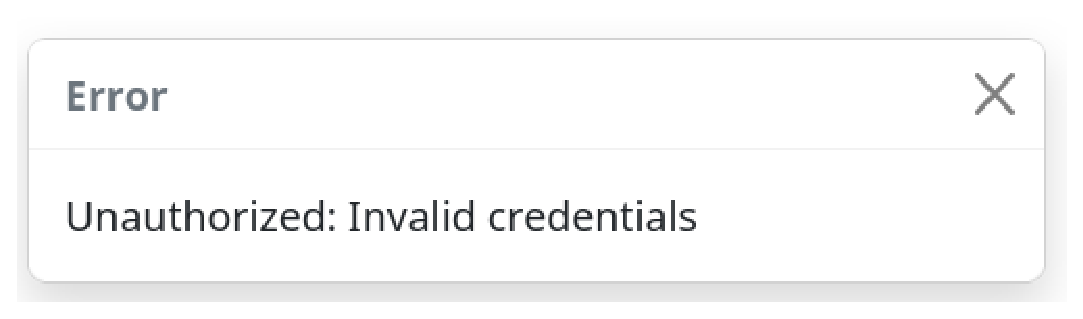
\includegraphics[width=\textwidth]{failedsignin}
  \caption{Informacja o niepoprawnych danych logowania}
  \label{atmosphere:failedsignin}
\end{figure}
Po udanym zalogowaniu w zależności od poziomu uprawnień użytkownik ma dostęp
do pozostałych zasobów aplikacji.
W tym samym momencie aplikacja łączy się z kanałem WebSocket odpowiedzialnym za
wysyłanie powiadomień o niespodziewanych wydarzeniach, tj. przekroczenie
wartości parametrów. Aby je utrzymać aplikacja wysyła wykorzystując te samo
połączenie wiadomość o treści "ping" co 30 sekund. W przypadku, gdy
wystąpi niespodziewane zdarzenie oraz kanał jest aktywny aplikacja otrzymuje
o tym wiadomość z serwera, a następnie wyświetlana jest w formacie powiadomienia
podobnym do wcześniej przedstawionego powiadomienia o nieudanym logowaniu.
Zawartość powiadomienia może zostać dynamicznie zmieniona przez użytkownika
jak i bardziej zaawansowana logika weryfikacji odczytów. Przykładowa konfiguracja
została przedstawiona na Rys. \ref{atmosphere:validation_rule}.
\begin{figure}[h!]
  \centering
  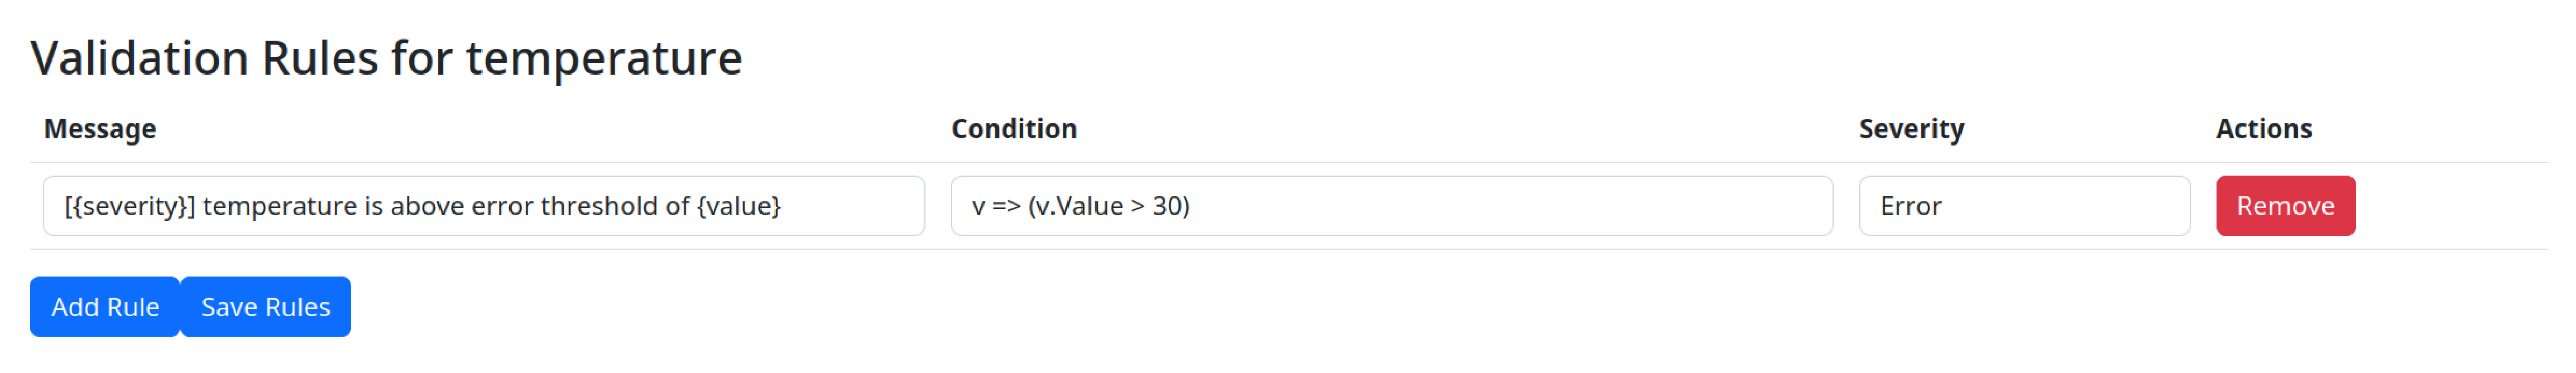
\includegraphics[width=\textwidth]{validation_rule}
  \caption{Przykładowa konfiguracja zasad walidacji}
  \label{atmosphere:validation_rule}
\end{figure}
Te reguły pozwalają na ustalenie dowolnej wiadomości opcjonalnie zawierającej referencje
do wartości odczytu (\textit{value}) oraz jego poziomu (\textit{severity}). Poziom może zostać
dostosowany przez użytkownika w zależności od priorytetu danej wiadomości.
Są one podzielone na trzy kategorie: informacje, ostrzeżenia oraz błędy.
Same reguły tworzone są za pomocą składni LINQ używanej w językach programowania
bazujących na środowisku .NET. Umożliwia to na konstrukcję bardziej zaawansowanych reguł
pozwalających na porównywanie wielu wartości, np. aplikacja może wysyłać powiadomienie, gdy
wartość odczytu przekroczy dany próg wyrażony w stopniach Celsjusza lub zupełnie inny
w stopnia Fahrenheita poprzez podanie dodatkowego porównania z polem jednostki (\textit{Unit}).
Przykład takiego wyrażenia przedstawiony został na Rys. \ref{atmosphere:custom_validation}.
\begin{figure}[h!]
  \centering
  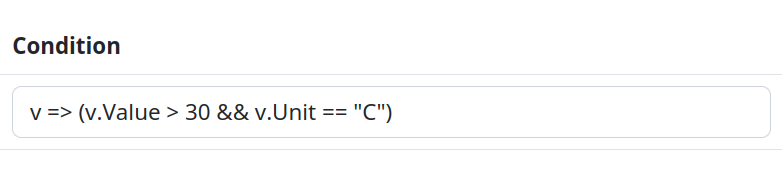
\includegraphics[width=\textwidth]{custom_validation}
  \caption{Przykładowa konfiguracja zasad walidacji ze specyfikacja jednostki}
  \label{atmosphere:custom_validation}
\end{figure}
Aplikacja umożliwia również konfigurację metody wysyłania powiadomień na adres email.
Administrator może skonfigurować takie parametry jak serwer SMTP oraz port wykorzystywany
do wysyłania wiadomości jak i nazwę użytkownika oraz hasło użyte do autoryzacji na nim.
Dodatkowo może on podać adres email, z którego dana wiadomość jest wysyłana jak i również
docelowy adres email. Przykładowa konfiguracja została zaprezentowana na Rys. \ref{atmosphere:email_configuration}.
\begin{figure}[h!]
  \centering
  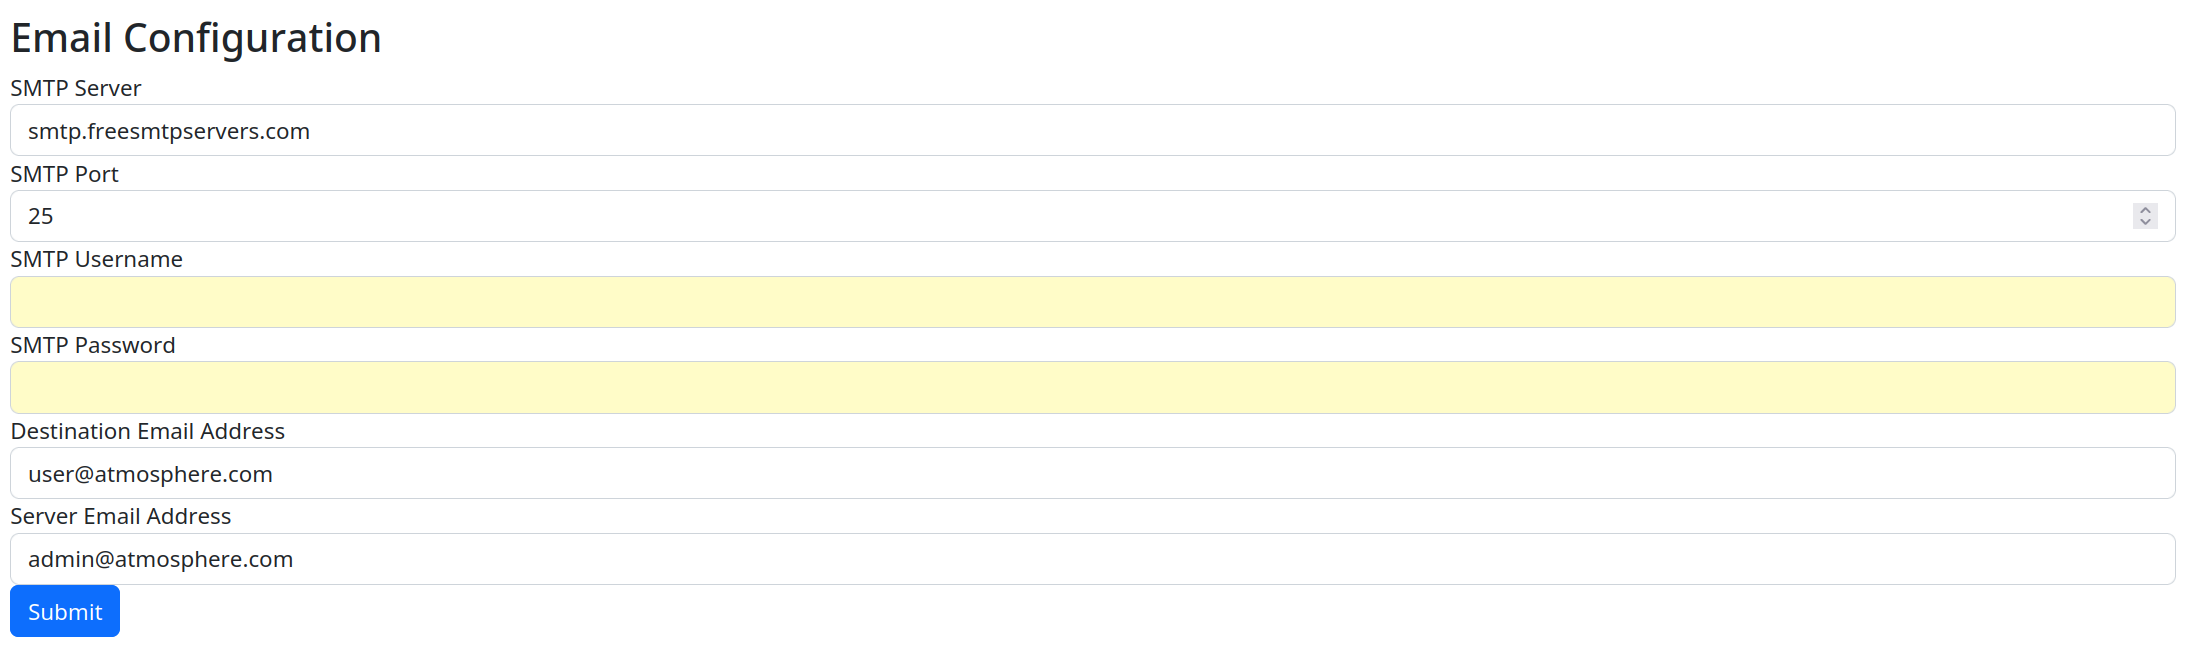
\includegraphics[width=\textwidth]{email_configuration}
  \caption{Przykładowa konfiguracja powiadomień email}
  \label{atmosphere:email_configuration}
\end{figure}

Kolejnym widokiem jest lista odczytów parametrów środowiska. Użytkownik może 
filtrować ją z użyciem daty startowej i/lub daty końcowej po czym uzyskuje
wyniki znajdujące się w tym przedziale. Przykład przefiltrowanych danych
został przedstawiony na rysunku \ref{atmosphere:readings}.
\begin{figure}[h!]
  \centering
  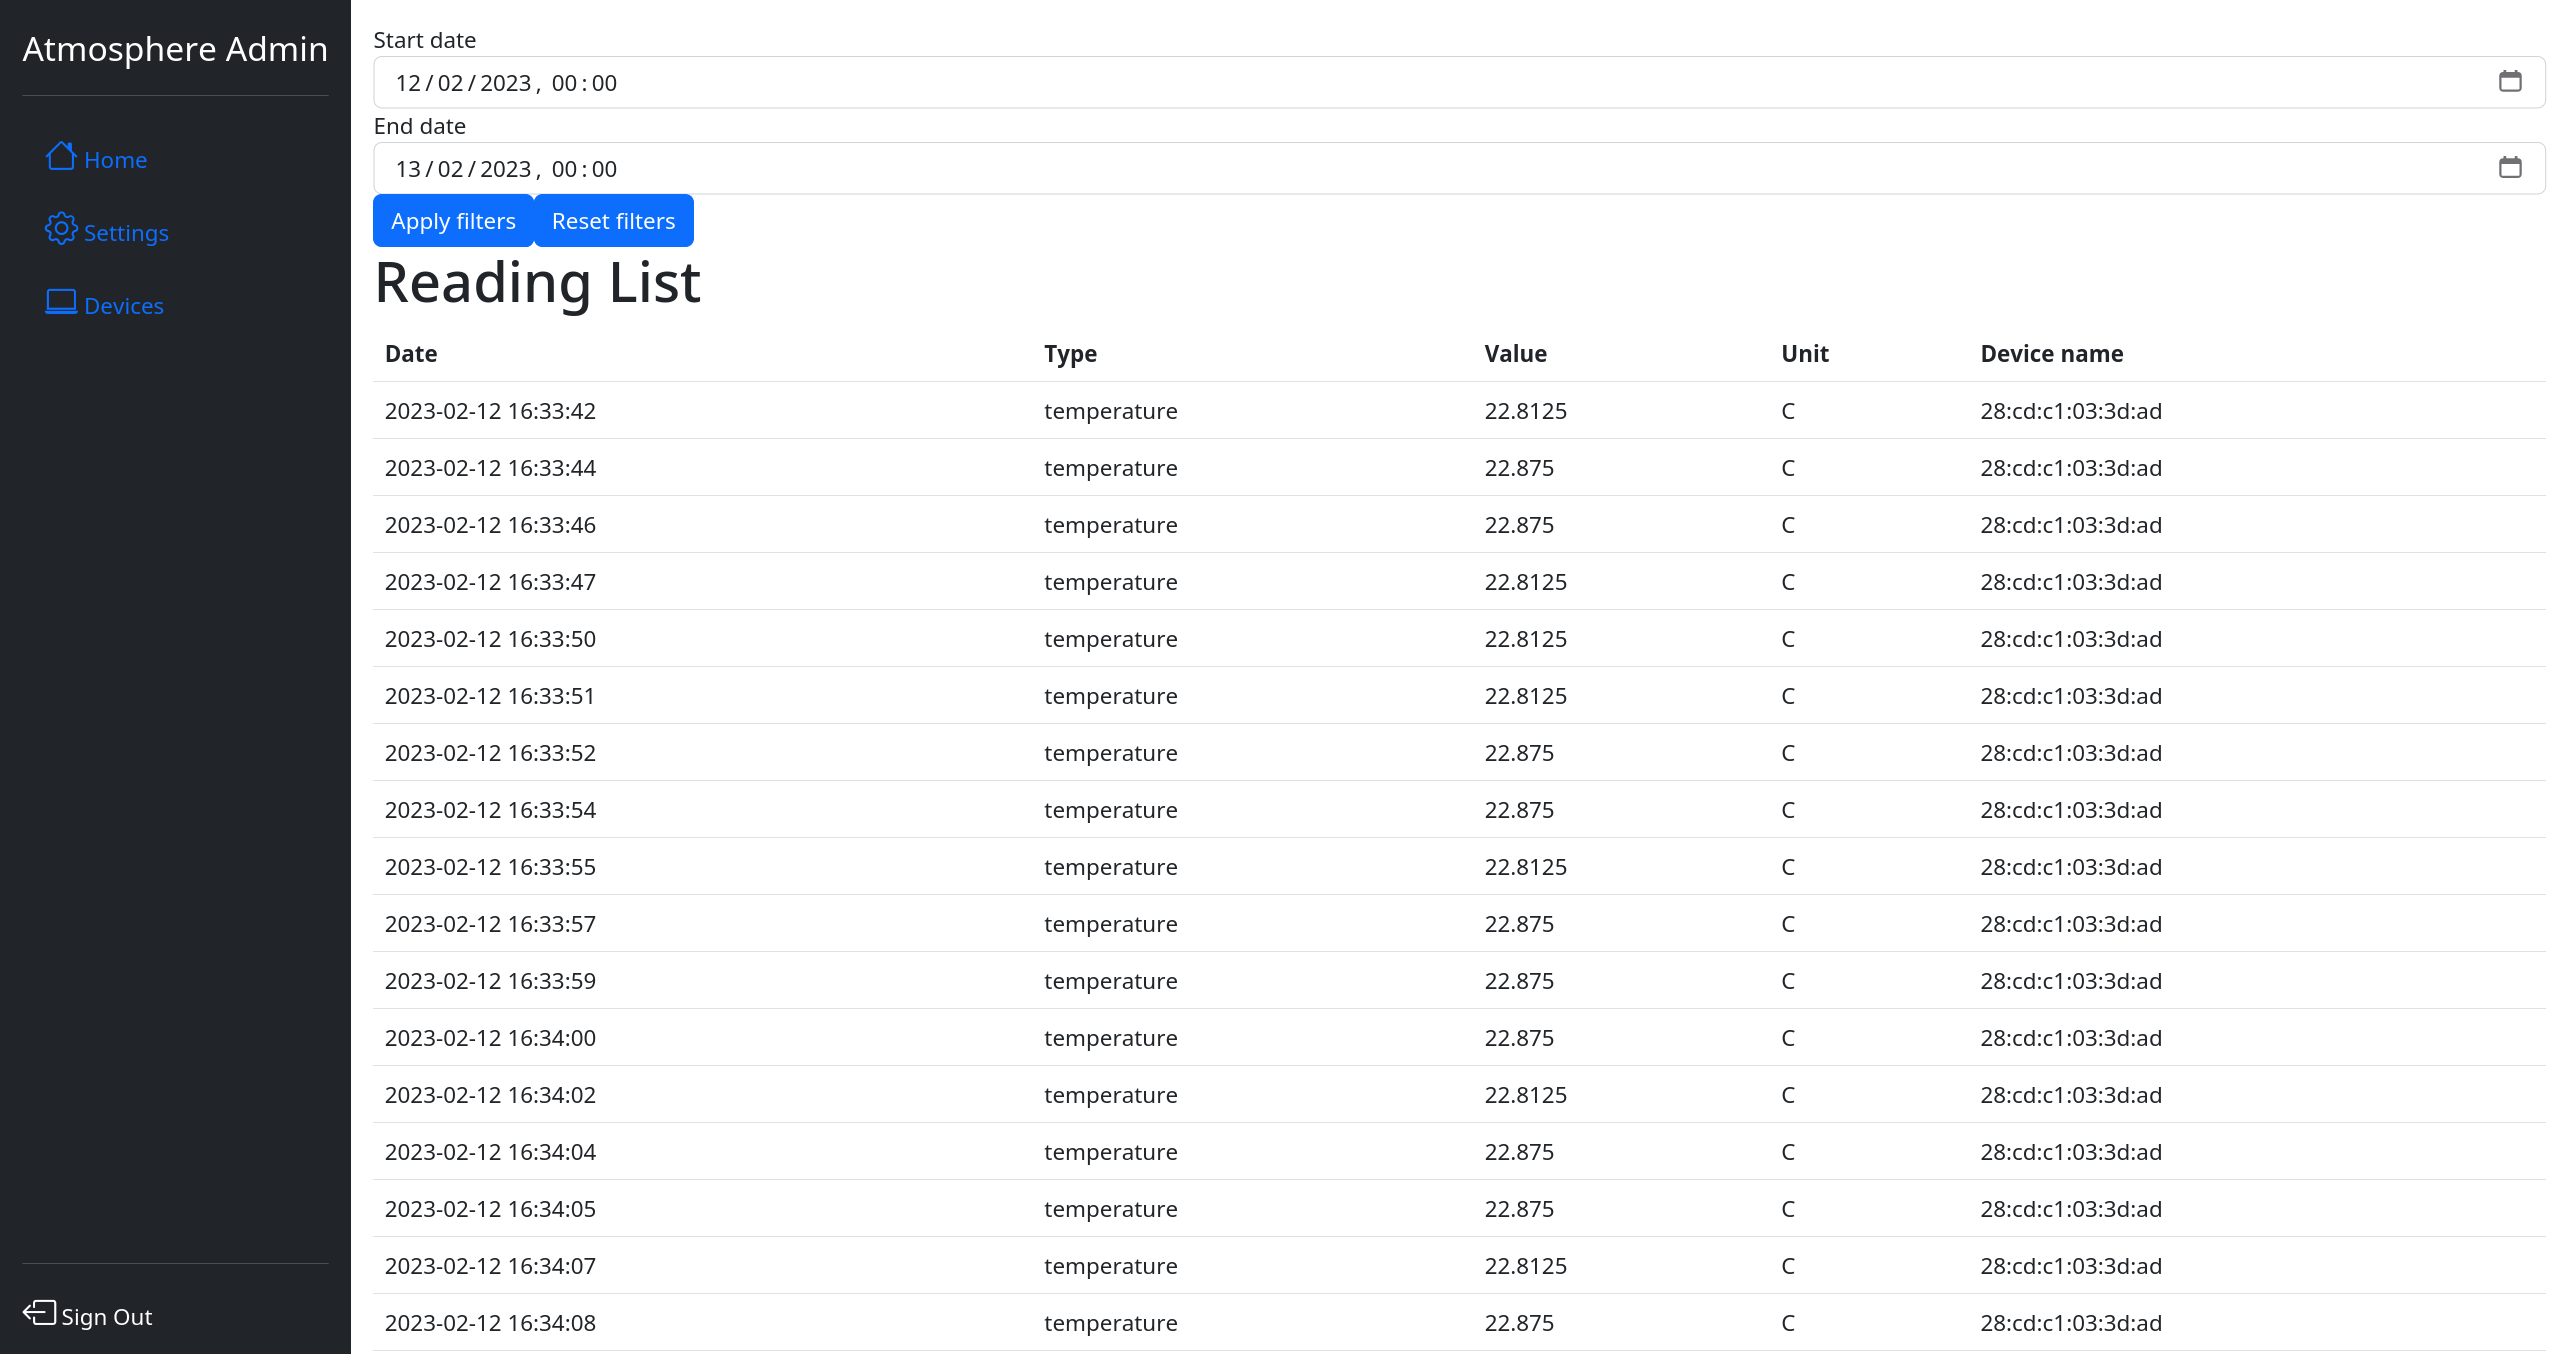
\includegraphics[width=\textwidth]{readings}
  \caption{Widok odczytów parametrów środowiska}
  \label{atmosphere:readings}
\end{figure}
Widok przedstawia w formie tabeli datę oraz czas wykonania odczytu, jego typ,
jednostkę pomiaru oraz adres fizyczny urządzenia pomiarowego.

\section{Urządzenie pomiarowe}
Do wykonywania pomiarów wykorzystany został mikrokontroler Raspberry Pi Pico W.
W celu uproszczenia tworzenia oprogramowania użyto nieoficjalnej implementacji
środowiska Arduino dla płytek z rodziny RP2040. Udostępnia ona prosty
w obsłudze poziom abstrakcji, który umożliwia na wykorzystanie głównych
możliwości mikrokontrolera takich jak odczyty z portów czy możliwość połączenia
z siecią bezprzewodową Wi-Fi. Możliwe jest dzięki temu również korzystanie z
wielu bibliotek stworzonych przez społeczność, które znacznie ułatwiają implementację.
Przykładem takiego modułu jest OneWire - biblioteka dodająca obsługę sensorów 
wykorzystujących jedną linię danych jako magistralę.
Jej wykorzystanie umożliwiło wykorzystanie jednej linii danych do połączenia wielu 
sensorów tej samej klasy.

W celu ułatwienia komunikacji z serwerem wykorzystana została zmodyfikowana wersja
generatora cpp-tiny znajdująca się w oprogramowaniu openapi-generator wykorzystując
wygenerowaną dokumentację OpenAPI 3.0. 
Ze względu na różnice w implementacji frameworku Arduino, aby uzyskać poprawnie 
wygenerowany kod zostały dokonane zmiany do plików mustache odpowiadających za składnię
generowanego kodu. W pliku Service.h.mustache, będącej nagłówkiem klasy odpowiadającej za komunikację z serwerem
oraz odpowiadającym serwisem, w celu usprawnionej obsługi nagłówków
HTTP oraz ich przechowywaniu do wykonania zapytania dodano zmienną przechowujące te nagłówki.
Podobnie, aby dostosować się do zmienionej logiki w pliku Service.cpp.mustache zmodyfikowane
zostało zapisywanie nagłówków - zamiast przechowywać je w kliencie HTTP, gdzie byłyby usuwane podczas
rozpoczęcia zapytania, przechowywane są we wcześniej stworzonej zmiennej, a następnie są one
wstrzykiwane klientowi zaraz po rozpoczęciu zapytania oraz przed jego wysłaniem.
Podobnie w przypadku pustych odpowiedzi wygenerowany kod nie był ich w stanie obsłużyć,
ze względu na implementację klienta HTTP, co kończyło się dostępem do niezmapowanej pamięci. 
Aby to rozwiązać w funkcji odpowiedzialnej 
za pobieranie odpowiedzi dodano dodatkowe zabezpieczenie w postaci sprawdzenia
długości odpowiedzi, jeżeli wynosi -1 odpowiedź jest o nieznanej długości i całość przepisywana jest
do bufora z wykorzystaniem potoku, w przypadku 0 odpowiedź jest pusta, a przy wartościach większych od
0 tworzony jest bufor o tej długości.

Podczas startu urządzenie łączy się z siecią Wi-Fi wcześniej zdefiniowaną przez użytkownika.
Jeżeli połączenie powiodło się następuje synchronizacja czasu z zewnętrznym serwerem NTP.
Zapewnia to spójność znaków czasu między urządzeniami w systemie, co wykorzystywane jest
przy procesowaniu pomiarów. Następnym krokiem jest inicjalizacja połączenia z serwerem.
Urządzenie najpierw próbuje przejść proces uwierzytelniania dostarczonym przez użytkownika
hasłem, jeżeli jest to pierwszy raz kiedy dane urządzenie łączy się z systemem tworzone jest
jemu nieaktywne konto, które następnie musi zostać zaakceptowane przez administratora.
Jeżeli wcześniejszy proces przebiegł z powodzeniem urządzenie kontynuuje do połączenia
z odpowiednim kanałem WebSocket po czym przechodzi do stanu normalnej operacji.

Aby zapewnić synchronizację z serwerem oraz dostęp do statusu połączenia wykorzystano
technologię WebSocket. Urządzenie łączy się z odpowiednim gniazdem, a następnie co 30
sekund wysyła wiadomość z zawartością "ping" i oczekuje na odpowiedź "pong" od serwera.
Jeżeli nie otrzyma takiej wiadomości uznaje, że połączenie zostało zerwane, więc zamyka je
i po upływie 5 sekund próbuje utworzyć ponowną komunikację. Dzieje się to aż do momentu przywrócenia
połączenia po czym urządzenie powraca do normalnego trybu operacji odczytywania oraz
przesyłania danych z sensorów.

Urządzenie pomiarowe, podczas normalnej operacji, dokonuje pomiarów z podłączonych sensorów, 
a następnie przetwarza je i w odpowiednim formacie wysyła na serwer. Odbywa się to poprzez
wykorzystanie metody POST jednego z kontrolerów. Dane pomiaru zawierają takie informacje jak
data i czas wykonania, wartość, jednostka oraz typ pomiaru. Do autoryzacji tego zapytania
wykorzystywany jest wcześniej wygenerowany token JWT. Następnie urządzenie odczekuje wcześniej
skonfigurowaną ilość czasu przed następnym pomiarem. Jest ona obliczana jako różnica czasu, który
został spędzony na aktualnym przejściu, a ustalonym przez użytkownika okresem. Jeżeli jest ona
większa od zera urządzenie wyczekuje wyliczony przedział czasu, a następnie kontynuuje pracę.
